\documentclass[tikz,border=6pt]{standalone}
\usepackage{amsmath}
\usetikzlibrary{arrows.meta,positioning,shapes.geometric,shapes.misc,fit,calc}

\begin{document}
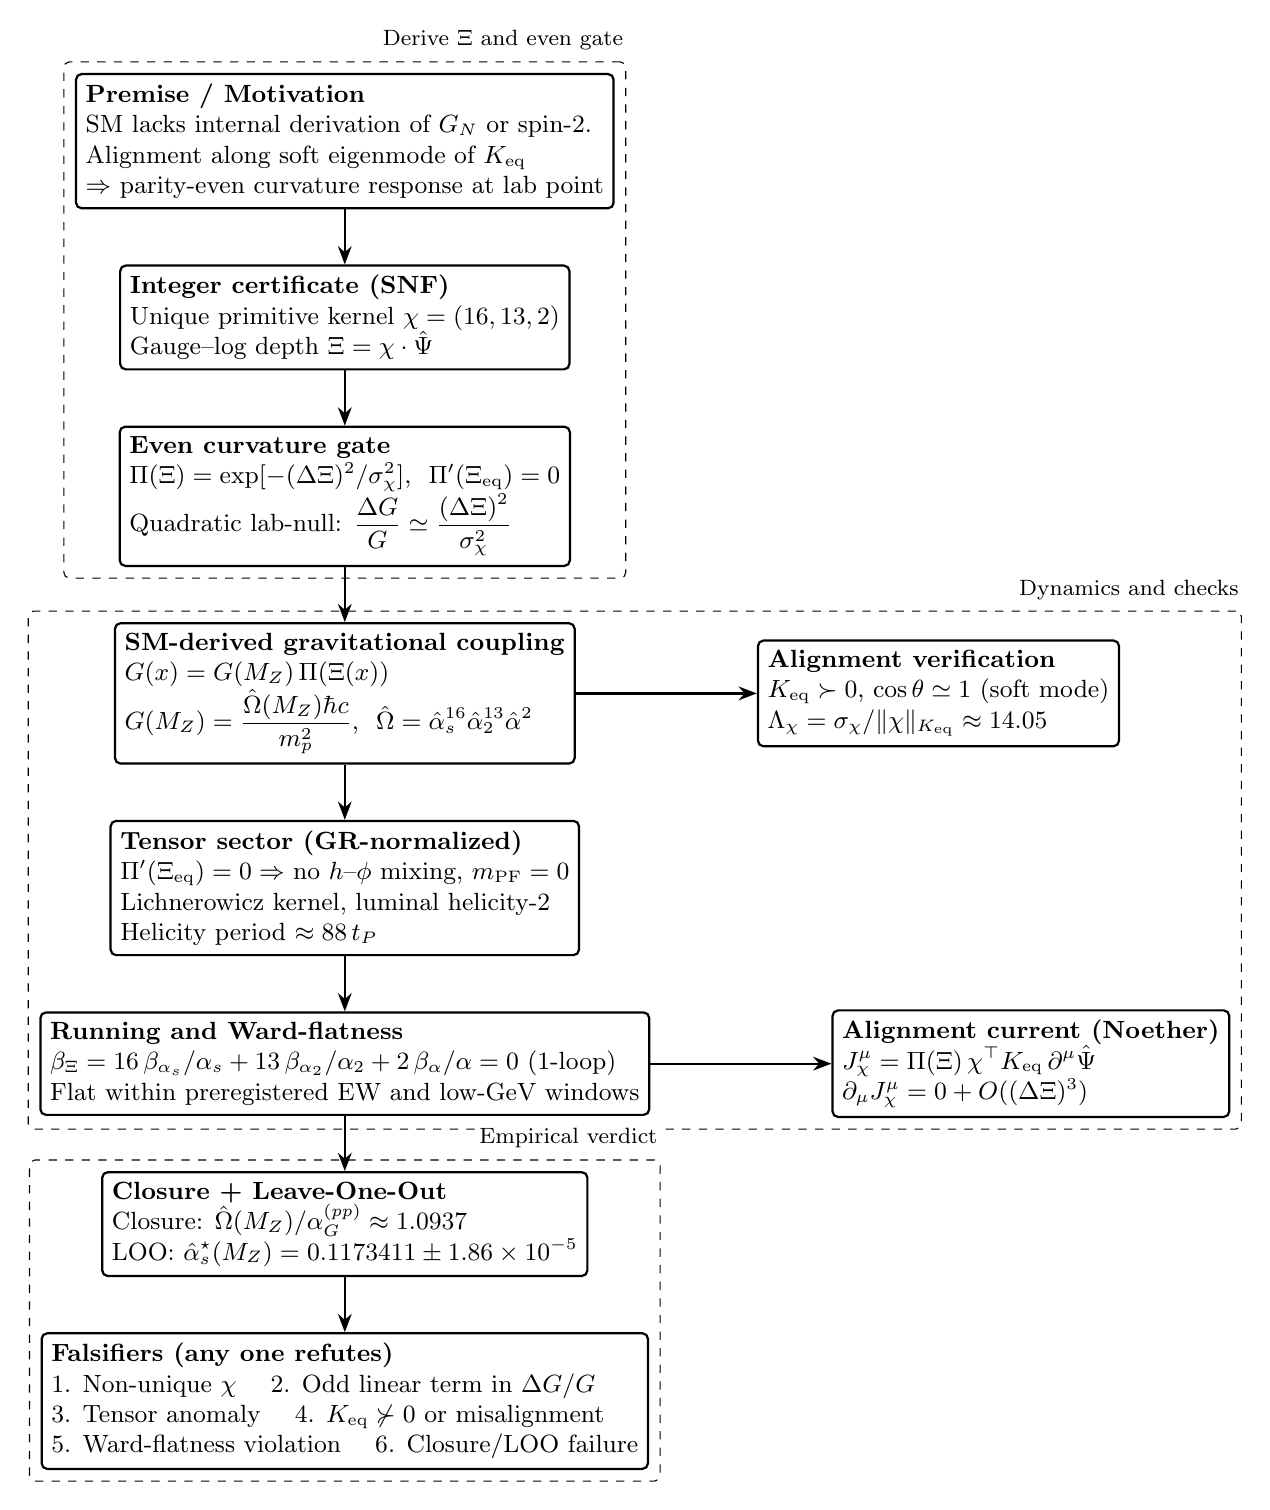
\begin{tikzpicture}[
  font=\small,
  node distance=7mm and 12mm,
  >={Stealth[length=2.2mm]},
  line/.style={-Stealth,thick},
  box/.style={rectangle, rounded corners=2pt, draw, thick, align=left, inner sep=3.5pt, fill=white},
  proc/.style={box, fill=white},
  test/.style={diamond, aspect=2.1, draw, thick, align=center, inner sep=2pt, fill=white},
  group/.style={rectangle, rounded corners=2pt, draw, dashed, inner sep=4pt}
]

% Nodes
\node[proc] (premise) {\textbf{Premise / Motivation}\\
SM lacks internal derivation of $G_N$ or spin-2.\\
Alignment along soft eigenmode of $K_{\rm eq}$\\
$\Rightarrow$ parity-even curvature response at lab point};

\node[proc, below=of premise] (certificate) {\textbf{Integer certificate (SNF)}\\
Unique primitive kernel $\chi=(16,13,2)$\\
Gauge--log depth $\Xi=\chi\cdot\hat\Psi$};

\node[proc, below=of certificate] (gate) {\textbf{Even curvature gate}\\
$\Pi(\Xi)=\exp[-(\Delta\Xi)^2/\sigma_\chi^2]$, \ $\Pi'(\Xi_{\rm eq})=0$\\
Quadratic lab-null: $\displaystyle \frac{\Delta G}{G}\simeq \frac{(\Delta\Xi)^2}{\sigma_\chi^2}$};

\node[proc, below=of gate] (Gdef) {\textbf{SM-derived gravitational coupling}\\
$G(x)=G(M_Z)\,\Pi(\Xi(x))$\\
$G(M_Z)=\dfrac{\hat\Omega(M_Z)\hbar c}{m_p^2}$, \ $\hat\Omega=\hat\alpha_s^{16}\hat\alpha_2^{13}\hat\alpha^2$};

\node[proc, right=23mm of Gdef] (align) {\textbf{Alignment verification}\\
$K_{\rm eq}\succ0$, $\cos\theta\simeq 1$ (soft mode)\\
$\Lambda_\chi=\sigma_\chi/\|\chi\|_{K_{\rm eq}}\approx 14.05$};

\node[proc, below=of Gdef] (tensor) {\textbf{Tensor sector (GR-normalized)}\\
$\Pi'(\Xi_{\rm eq})=0 \Rightarrow$ no $h$--$\phi$ mixing, $m_{\rm PF}=0$\\
Lichnerowicz kernel, luminal helicity-2\\
Helicity period $\approx 88\,t_P$};

\node[proc, below=of tensor] (running) {\textbf{Running and Ward-flatness}\\
$\beta_\Xi = 16\,\beta_{\alpha_s}/\alpha_s + 13\,\beta_{\alpha_2}/\alpha_2 + 2\,\beta_\alpha/\alpha = 0$ (1-loop)\\
Flat within preregistered EW and low-GeV windows};

\node[proc, below=of running] (closure) {\textbf{Closure + Leave-One-Out}\\
Closure: $\hat\Omega(M_Z)/\alpha_G^{(pp)} \approx 1.0937$\\
LOO: $\hat\alpha_s^\star(M_Z)=0.1173411\pm 1.86\times 10^{-5}$};

\node[proc, right=23mm of running] (current) {\textbf{Alignment current (Noether)}\\
$J_\chi^\mu=\Pi(\Xi)\,\chi^\top K_{\rm eq}\,\partial^\mu\hat\Psi$\\
$\partial_\mu J_\chi^\mu=0 + O((\Delta\Xi)^3)$};

\node[proc, below=of closure] (falsifiers) {\textbf{Falsifiers (any one refutes)}\\
1. Non-unique $\chi$ \quad 2. Odd linear term in $\Delta G/G$\\
3. Tensor anomaly \quad 4. $K_{\rm eq}\not\succ0$ or misalignment\\
5. Ward-flatness violation \quad 6. Closure/LOO failure};

% Arrows (main spine)
\draw[line] (premise) -- (certificate);
\draw[line] (certificate) -- (gate);
\draw[line] (gate) -- (Gdef);
\draw[line] (Gdef) -- (tensor);
\draw[line] (tensor) -- (running);
\draw[line] (running) -- (closure);
\draw[line] (closure) -- (falsifiers);

% Side links
\draw[line] (Gdef.east) -- (align.west);
\draw[line] (running.east) -- (current.west);

% Optional groups (visual clustering)
\node[group, fit=(premise)(certificate)(gate)] (grp1) {};
\node[group, fit=(Gdef)(align)(tensor)(running)(current)] (grp2) {};
\node[group, fit=(closure)(falsifiers)] (grp3) {};

\node[above left=1mm and 0mm of grp1.north east, anchor=south east, fill=white, inner sep=1pt] {\footnotesize Derive $\Xi$ and even gate};
\node[above left=1mm and 0mm of grp2.north east, anchor=south east, fill=white, inner sep=1pt] {\footnotesize Dynamics and checks};
\node[above left=1mm and 0mm of grp3.north east, anchor=south east, fill=white, inner sep=1pt] {\footnotesize Empirical verdict};

\end{tikzpicture}
\end{document}
